\documentclass[reqno]{amsart}

\usepackage{external/takodachi}

\renewcommand{\emph}[1]{\textsc{#1}}

\title
{
	{Littlewood-Paley theory}
} 

\author{Jason Zhao}
\date{\today}

\begin{document}
\maketitle

\begin{abstract}
	The Littlewood-Paley projections separate the frequencies of a function in a quantitative manner, reducing the study of a generic function to that of its frequency-localised pieces. These notes take inspiration from \cite{Tao2006}, \cite{BahouriEtAl2011}, \cite{Stein16}, \cite{Grafakos2014a}. 
\end{abstract}

\tableofcontents

\section{Littlewood-Paley projections}
Before getting into any multi-linear algebra, it is important to get a grasp of coordinates in linear algebra and how these coordinates respond to change of bases. Let $V$ be an $n$-dimensional real vector space, and denote $V^*$ its dual space. Given a basis $\{e_i\}_i \subseteq V$, there exists a dual basis $\{\epsilon^j\}_j \subseteq V^*$ satisfying 
	\[ \langle e_i, \epsilon^j \rangle = \delta^j_i. \]
Choose another basis $\{\widetilde e_i\}_i \subseteq V$ and denote its dual basis by $\{\widetilde \epsilon^j\}_j \subseteq V^*$. There exists a change of basis matrix $C^k_i \in \mathsf{GL} (\R^n)$ sending the original basis to the new basis,
	\[ \widetilde e_i = C^k_i e_k. \]	
On the other hand, the inverse change of basis matrix $(C^{-1})^j_k \in \mathsf{GL} (\R^n)$, i.e. $(C^{-1})^j_k C^k_i = \delta^j_i$, transforms the original dual basis to the new dual basis 	
	\[ \widetilde \epsilon^j = (C^{-1})^j_k \epsilon^k. \]
Throughout these notes, we will use these \emph{Einstein summation notation}, where repeated indices are summed over, e.g. $a^i b_i := \sum_i a^i b_i$.


\subsection{{Contravariance}}

We say an object is \emph{contravariant} if the coordinate representation \textit{contra-varies} with respect to change of basis, that is, transforms by the inverse matrix $(C^{-1})^j_i$. Such coordinates are indexed by \textit{upper indices}. The prototypical example of a contravariant object is a \emph{vector} $v \in V$. Every vector admits a unique coordinate representation $\{v^i\}_i \subseteq \R$ with respect to the basis $\{e_i\}_i$, i.e.
	\[ v = v^i e_i . \]
Let $\{ \widetilde v^j \}_j \subseteq \R$ be the unique coordinates with respect to the basis $\{\widetilde e_j\}_j$, then the change of coordinates from $\{v^i\}_i$ to $\{\widetilde v^j\}_j$ is given by the inverse change of basis matrix,
	\[ \widetilde v^j = {(C^{-1})}^j_i v^i. \]
Indeed, 	
	\[ v = \widetilde v^j \widetilde e_j  = \left( {(C^{-1})}^j_i v^i \right) \left( C^k_j e_k \right) = \delta^k_i v^i e_k = v^i e_i . \]
We can interpret a choice of basis $\{e_i\}_i$ as endowing $V$ with a ``measuring tool'', where the coordinates $\{v^i\}_i$ representing the resulting ``measurement''. A change of basis corresponds to changing the choice of ``measuring tool'', e.g. we can view a change of basis $\widetilde e_i = \tfrac{1}{100} e_i$ as changing from ``meters'' $e_i$ to ``centimeters'' $\widetilde e_i$, so the corresponding change of coordinates is 
	\[ \widetilde v^i \text{ meters } = 100 v^i \text{ centimeters}. \]




\subsection{Covariance}

We say that an object is \emph{covariant} if the coordinate representation \textit{co-varies} with respect to change of basis, that is, transforms by the matrix $C^k_i$.  Such coordinates are indexed by \textit{lower indices}. The prototypical example of a covariant object is a \emph{covector} $\omega \in V^*$. Every covector admits a unique coordinate representation $\{\omega_i \}_i \subseteq \R$ with respect to the basis $\{\epsilon^i\}_i$, i.e.
	\[ \omega = \omega_i \epsilon^i = \widetilde \omega_j \widetilde \epsilon^j. \]
Let $\{\widetilde \omega_j \}_j \subseteq \R$ be the unique coordinates with respect to the basis $\{\widetilde \epsilon^j\}_j$, then the change of coordinates from $\{\omega_i\}_i$ to $\{\widetilde \omega_j\}_j$ is given by the change of basis matrix,
	\[ \widetilde \omega_j = C^i_j \omega_i \]
Indeed, 
	\[ \omega = \widetilde \omega_j \widetilde \epsilon^j = \left( C^i_j \omega_i \right) \left( (C^{-1})_k^j \epsilon^k \right) =  \delta^i_k \omega_i \epsilon^k = \omega_i \epsilon^i. \]
Scalars are regarded as ``dimensionless'' quantities, so since a covector acting on a vector produces a scalar, they have inverse dimensions. For example, we can view a change of basis $\widetilde \epsilon^j = 100 \epsilon^j$ as changing from  ``meters$^{-1}$'' $\epsilon^j$ to ``centimeters$^{-1}$'' $\widetilde \epsilon^j$, so the corresponding change of coordinates is 
	\[ \widetilde \omega_j \text{ meters$^{-1}$} = \frac{1}{100} \omega_j  \text{ centimeters$^{-1}$}. \]



\section{Convergence of $P_{1/N \leq - \leq N}$ and $P_{\leq N}$}
If we want to reduce the study of tempered distributions or functions to that of their Littlewood-Paley pieces, we need to figure out under what conditions and which topologies do the following limits hold, 
	\[ f = \lim_{N \to \infty} f_{\leq N} , \qquad f = \lim_{N \to \infty} f_{1/N \leq - \leq N} . \]
We refer to the former as the limit of  \textit{inhomogeneous} projections, and the latter as the sum of \textit{homogeneous projections}, abbreviating
	\[ \sum_{N \in 2^\Z} := \lim_{N \to \infty} f_{1/N \leq - \leq N}. \]


\subsection{$\cS$ and $\cS^*$-convergence}

The natural starting point is the weakest topology in which these projections could converge: the topology of tempered distributions. By duality, this would follow from proving convergence in the Schwartz topology, which is a straight-forward application of dominated convergence. 

\begin{proposition}[Inhomogeneous projections on $\cS (\R^d)^*$]
	Let $f \in \cS (\R^d)$ be a Schwartz function, then 
		\[ f = \lim_{N \to \infty} f_{\leq N} \]
	in the sense of Schwartz functions. Dually, if $f \in \cS (\R^d)^*$ is a tempered distribution, then the limit holds in the sense of tempered distributions. 
\end{proposition}

\begin{proof}
	Since the Fourier transform is an isomorphism, the inhomogeneous projections converge $P_{\leq N} f \to f$ in the $\cS (\R^d)$-topology if and only if $\phi_{\leq N} \widehat f \to \widehat f$ also converge in $\cS (\R^d)$-topology. Fix a Schwartz semi-norm indexed by multi-indices $\alpha, \beta \in \N^d_0$, we write using the Leibniz rule
		\begin{align*}
			 ||\xi^\alpha \Big( \partial^\beta (1 - \phi_{\leq N}) \widehat f \Big) ||_{L^\infty}
			 	&\lesssim ||\xi^\alpha (1 - \phi_{\leq N})\partial^\beta \widehat f||_{L^\infty} +  \sum_{0 < \gamma \leq \beta}||\xi^\alpha \partial^{\gamma}  \phi_{\leq N} \partial^{\beta - \gamma} \widehat f ||_{L^\infty} .
		\end{align*}	 
	Here we used the triangle inequality to split between the cases where the derivatives only hit $\widehat f$ and when derivatives hit $1 - \phi_{\leq N}$. In the former case, the multiplier $1 - \phi_{\leq N}$ is supported on $|\xi| \gtrsim N$, so the first term on the right vanishes under the limit by rapid decay of $\partial^\beta \widehat f \in \cS (\R^d)$. In the latter case, we compute
		\[ \partial^\gamma \phi_{\leq N} (\xi) = N^{-|\gamma|} \partial^\gamma \phi (\xi/N). \]
	As $|\partial^\gamma \phi|, |\xi^\alpha \partial^{\beta - \gamma} \widehat f| \lesssim 1$, the decay from the negative powers of $N$ shows the second term on the right vanishes.
	
	For tempered distributions $f \in \cS (\R^d)^*$, the inhomogeneous projections converge pointwise and thus in the $\cS (\R^d)^*$-topology. This follows from self-adjointness of the projections and continuity of tempered distributions, 
		\begin{align*}
			\lim_{N \to \infty}\langle  g, P_{\leq N} f \rangle = \lim_{N \to \infty} \langle P_{\leq N} g, f \rangle = \langle g, f \rangle
		\end{align*}
	for every $g \in \cS (\R^d)$. 
\end{proof}

\subsection{Homogeneous spaces}

Formally, the linear map
	\[ f \mapsto \sum_{N \in 2^\Z} f_N \]
has non-trivial kernel, namely the tempered distributions with Fourier transform supported at the origin. These are precisely the polynomials $\mathcal P (\R^d)$, so any hope of proving convergence in the homogeneous case must be up to polynomials. Moreover, this map isn't even well defined! We write $(1 - P_{1/N \leq - \leq N}) f$ in frequency space as the sum of a \textit{low frequency tail} and \textit{high frequency tail},
	\[ (1 - \psi_{1/N \leq - \leq N}) \widehat f = \phi_{\leq 1/N} \widehat f + (1 - \phi_{\leq N}) \widehat f .\]
Let $f \in \cS (\R^d)$, and consider the Schwartz semi-norms. The high frequencies are dealt with exactly as in the inhomogeneous case. The problem arises when derivatives hit the low frequencies, as $\partial^\beta \phi_{\leq 1/N} (x) = N^{|\beta|} \partial^\beta \phi(Nx)$ grows in amplitude as $N \to \infty$. To get around this issue, note $\phi_{\leq 1/N}$ is supported at frequencies $|\xi| \lesssim 1/N$, so multiplying by a function which vanishes to infinite order allows us to ``defeat'' this growth via Taylor's theorem. 

Define the \emph{homogeneous Schwartz space} $\dot \cS (\R^d)$ as the space of Schwartz functions whose Fourier transform vanishes to every order at the origin, 
	\[\dot \cS (\R^d) := \{ f \in \cS (\R^d) : \nabla^k \widehat f (0) = 0 \text{ for every $k$} \}. \]
As expected from our initial remark, the dual space is the space of tempered distributions modulo the space of polynomials $\mathcal P (\R^d)$.

\begin{proposition}
	The dual space of the homogeneous Schwartz space is
		\[ \dot \cS (\R^d)^* = \cS(\R^d)^* / \mathcal P (\R^d). \]
\end{proposition}

\begin{proof}
	Define $T: \cS (\R^d)^* \to \dot \cS (\R^d)^*$ be the restriction map
		\[ T u := u_{|\dot \cS (\R^d)}.  \]
	We claim that the restriction map is surjective and the kernel is precisely the space of polynomials. The first isomorphism theorem furnishes the result. Surjectivity follows from Hahn-Banach, so it remains to study the kernel. 	Suppose $u \in \operatorname{ker} T$, then by Plancharel 
		\[ 0 = \langle u, \phi \rangle = \langle \widehat u, \widehat \phi \rangle \]
	for all $\phi \in \dot \cS (\R^d)$. Since $\widehat \phi$ vanishes to infinite order at the origin, it follows that $\widehat u$ must be supported at the origin. Such distributions are derivatives of the Dirac mass at the origin, which upon applying the Fourier inverse shows that $u$ is a polynomial. 
\end{proof}	

\begin{proposition}[Homogeneous projections on $\dot \cS (\R^d)^*$]
	Let $f \in \cS (\R^d)$ be a Schwartz function, then 
		\[ f = \sum_{N \in 2^\Z} f_N \]
	in the sense of Schwartz functions if and only if $f \in \dot \cS (\R^d)$. Dually, if $f \in \cS (\R^d)$ is a tempered distribution, then the series holds in the sense of tempered distributions up to polynomials. 	
\end{proposition}

Of course, we are interested in the theory of tempered distributions for the sake of studying partial differential equations. It's quite technically annoying and unsatisfying to solve an equation in a quotient space, so one might ask under what conditions does the formula $f = \sum_N f_N$ hold? 

\begin{proposition}[Homogeneous projections on $\cS (\R^d)^*$]
	Let $f \in \cS(\R^d)^*$, then 
		\[ f = \sum_{N \in 2^\Z} f_N \]
	in the sense of tempered distributions if and only if the low frequency tail vanishes in the sense of tempered distributions,
		\[ \lim_{N \to \infty} f_{\leq 1/N} = 0. \]	
\end{proposition}

\begin{remark}
	Failure of convergence for low frequencies is sometimes known as \textit{infrared divergence}. 
\end{remark}

Define the space of tempered distributions for which the representation formula $f = \sum_N f_N$ holds by 
	\[ \cS_h^* := \{ f \in \cS (\R^d)^* :  \lim_{N \to \infty} f_{\leq 1/N} = 0\}.  \]
The low frequency projections act identically on polynomials, so this space does not contain any polynomials, which were the main obstruction to the representation formula from holding. However, we have to pay a price for this formula; this is not a closed subspace of $\cS (\R^d)^*$. For example, take any $f \in \cS (\R^d)$ such that $f (0) = 1$, then the rescalings $f_n (x) := f(x/n)$ converge to the constant function $1$. 
\begin{example}
	The following are sufficient conditions for $f \in \cS_h^*$:
\begin{itemize}
		\item $||f_{\leq 1/N}||_{L^\infty} \to 0$ since the $L^\infty$-topology is stronger than the $\cS^*$-topology. This is the approach taken by \cite{BahouriEtAl2011} in the interest of \textit{realising} the homogeneous Besov spaces. 
		
		\item $\widehat f$ is locally integrable near the origin. In particular, the space of compactly supported distributions is a subspace, $C^\infty (\R^d)^* \subseteq \cS^*_h$. 
\end{itemize}
\end{example}	




\subsection{$L^p$-convergence}

We prove the projections converge to $f \in L^p (\R^d)$ in the norm topology modulo modifications at the endpoints $p = 1, \infty$. This is particularly useful in the homogeneous case $f = \sum_N f_N$, as it allows us to use the triangle inequality with impunity and estimate
	\[ ||f||_{L^p} \leq \sum_{N \in 2^\Z} ||f_N||_{L^p} .\]
playing into the philosophy that if one wants to study $f$, it suffices to study each of its Littlewood-Paley pieces. 

\begin{proposition}[$L^p$-boundedness]
	Let $1 \leq p \leq \infty$, then 
		\[||f_N||_{L^p}  \lesssim ||f||_{L^p},\]	
	uniformly for $f \in L^p (\R^d)$ and $N \in 2^\Z$. The analogous inequality holds replacing $f_N$ with $f_{\leq N}$. \label{prop:bounded}
\end{proposition}

\begin{proof}
	We prove the results for $f_N$, the proof is analogous for $f_{\leq N}$. It follows from Young's convolution inequality and a change of variables $Nx = y$ that 
		\[ ||f_N||_{L^p} = || f * \widecheck{\psi_N} ||_{L^p} \leq ||f||_{L^p} ||N^d \widecheck \psi (Nx)||_{L^1_x} = ||f||_{L^p} ||\widecheck \psi (y) ||_{L^1_y}. \] 
	This proves boundedness in $L^p (\R^d)$. 
\end{proof}

\begin{proposition}[$L^p$-convergence, non-endpoint]
	Let $1 < p < \infty$ and $f \in L^p (\R^d)$, then
		\[ f = \lim_{N \to \infty} f_{\leq N} = \sum_{N \in 2^\Z} f_N \]
	in $L^p$-norm. \label{prop:converge}
\end{proposition}

\begin{proof}
	By Plancharel and dominated convergence, the result clearly hold for $p = 2$. For $p \neq 2$, we first show convergence in $L^p$-norm for Schwartz $f \in \cS (\R^d)$ via interpolation, and then extend to general $L^p$-functions by density. Consider the case where $1 < p < 2$, and let $0 < \theta < 1$ satisfy $\tfrac1p = \tfrac{\theta}{1} + \tfrac{1 - \theta}{2}$, then 
		\begin{align*}
			 ||f_{\leq N} - f||_{L^p} 
					 	&\leq ||f_{\leq N} - f||_{L^1}^\theta ||f_{\leq N} - f||_{L^2}^{1 - \theta}\\
					 	& \lesssim ||f||^\theta_{L^1}||f_{\leq N} - f||_{L^2}^{1 - \theta} \overset{N \to \infty}{\longrightarrow} 0. 
		\end{align*}
	In the case $2 < p < \infty$, let $0 < \theta < 1$ satisfy $\tfrac1p = \tfrac\theta2 + \tfrac{1 - \theta}{\infty}$, then 
				\begin{align*}
					 ||f_{\leq N} - f||_{L^p} 
					 	&\leq ||f_{\leq N} - f||_{L^2}^\theta ||f_{\leq N} - f||_{L^\infty}^{1 - \theta}\\
					 	& \lesssim ||f_{\leq N} - f||_{L^2}^{\theta}   ||f||^{1 - \theta}_{L^\infty}\overset{N \to \infty}{\longrightarrow} 0. 
				\end{align*}	
	Suppose now $f \in L^p (\R^d)$, then for every $\epsilon > 0$ there exists $g \in \cS (\R^d)$ such that $||f - g||_{L^p} < \epsilon$. By the triangle inequality and convergence in $L^p$-norm for Schwartz functions, we have 
		\begin{align*}
			||f_{\leq N} - f ||_{L^p} 								&\leq || g_{\leq N} - g||_{L^p} + ||f - g||_{L^p} + ||(f - g)_{\leq N}||_{L^p}\lesssim \epsilon.
		\end{align*}		
	for $N \gg 1$. 	
\end{proof}

At the $p = \infty$ endpoint, we recall from Paley-Wiener that each Littlewood-Paley piece is analytic and thus continuous. Continuous functions form a closed subspace of $L^\infty (\R^d)$, so continuity is a necessary condition for convergence to hold in the uniform topology. 

\begin{proposition}[$L^\infty$-convergence]
	Let $f \in C_0 (\R^d)$, then
		\[ f = \lim_{N \to \infty} f_{\leq N} = \sum_{N \in 2^\Z} f_N \]
	in $L^\infty$-norm. Conversely, if $f \in L^\infty (\R^d)$ and the limit holds, then $f$ is continuous. \label{prop:inftyconv}
\end{proposition}

\begin{proof}
	As in the $L^p$-case, to show convergence it suffices to show the result for $f \in \cS (\R^d)$ as the Schwartz space is dense in $C_0 (\R^d)$ in the uniform topology. In place of interpolation, we instead use the $L^1 \to L^\infty$-inequality of the Fourier transform and dominated convergence,
		\[ || f_{\leq N} - f||_{L^\infty} \leq || \phi_{\leq N} \widehat f - \widehat f||_{L^1} \overset{N \to \infty}{\longrightarrow} 0. \]
	Conversely, if the limit holds, then $f$ must be continuous, since the Littlewood-Paley projections are continuous and continuity is preserved under uniform limits. 	
\end{proof}

At the endpoint $p = 1$, the Fourier integrals of $f \in L^1 (\R^d)$ are well-defined. In particular, the mean is given precisely by the contribution from frequency zero, $\int f = \widehat f (0)$. Thus the homogeneous projections $f_{1/N \leq - \leq N}$ have mean zero, which if they converge to $f$ in $L^1$-norm would imply $f$ also has mean zero.  Again, we see a difference between the homogeneous and inhomogeneous cases due to low frequencies. 

\begin{proposition}[$L^1$-convergence]
	Let $f \in L^1 (\R^d)$, then 
		\[ f = \lim_{N \to \infty} f_{\leq N} \]
	in $L^1$-norm. In the homogeneous case, convergence holds
		\[ f = \sum_{N \in 2^\Z} f_N \]
	in $L^1$-norm if and only if $\int f = 0$. 
\end{proposition}

\begin{proof}
	By density, let us assume $f \in C^\infty_c (\R^d)$, in which case by Proposition \ref{prop:inftyconv} we know convergence holds pointwise. It follows from Fatou's lemma and the triangle inequality that 
		\[ ||f_{\leq N} - f||_{L^1} \leq \sum_{K \geq N} ||f_K||_{L^1} \]
	and 
		\[ ||f_{1/N \leq - \leq N} - f||_{L^1} \leq ||f_{\leq 1/N}||_{L^1} + \sum_{K \geq N} ||f_K||_{L^1} . \]
	For the high frequency terms $K \geq N$, we can gain decay in the sum by paying a derivative on $f$ via the Sobolev-Bernstein inequality,
		\[ \sum_{K \geq N} ||f_K||_{L^1} \sim \sum_{K \geq N} K^{-1} || |\nabla| f_K||_{L^1} \lesssim \sum_{K \geq N} K^{-1} || |\nabla| f||_{L^1} \sim N^{-1} || |\nabla| f||_{L^1} \overset{N \to \infty}{\longrightarrow} 0.\]
	This proves the inhomogeneous case. To finish the proof of the homogeneous case, we similarly get decay of the low frequency terms by paying a derivative now on the kernel of the projection. More precisely, assume $\int f = 0$,  we can then write pointwise
		\begin{align*}
			 f_{\leq 1/N} (x) = (f * \widecheck{\phi_{\leq 1/N}})(x)
				&= N^{-d} \int_{\R^d} f(y)   \widecheck \phi(N^{-1} (x - y))  \, dy \\
				&= N^{-d} \int_{y \in \supp f} f(y)  \Big( \widecheck \phi(N^{-1} (x - y)) - \widecheck \phi(N^{-1} x) \Big) \, dy\\							&= N^{-d} \int_{y \in \supp f} f(y)  \Big(N^{-1} y \cdot \int_0^1 \nabla \widecheck \phi(N^{-1} x - \theta N^{-1} y )\, d \theta \Big) \, dy,
		\end{align*}
	where we use the mean-zero condition in the second line and the fundamental theorem of calculus in the third line. We can estimate the inner integrand $|\nabla \widecheck \phi (N^{-1} x - \theta N^{-1}y)| \lesssim_f \langle N^{-1} x \rangle^{-100d}$, since $y$ is in the compact support of $f$ and $\nabla \widecheck \phi \in \cS (\R^d)$. Taking the $L^1$-norm of the above, we obtain
			\begin{align*}
				||f_{\leq 1/N} ||_{L^1}								&\lesssim N^{-d - 1} \int_{\R^d} \int_{y \in \supp f} \frac{|y|}{\langle N^{-1}x \rangle^{100d}}|f(y)| dy dx   \sim_{f, d} N^{-1} \overset{N \to \infty}{\longrightarrow} 0,
					\end{align*}	
	as desired. To show necessity of the mean-zero condition, note that $\int f_{1/N \leq - \leq N} = \widehat{f_{1/N \leq - \leq N}} (0) = 0$, so convergence in $L^1$-norm would imply that $\int f = 0$. 
\end{proof}	




\section{Estimates}
The Littlewood-Paley projections separate in a quantitative manner the different frequencies of a function or tempered distribution. We can describe this separation qualitatively by the following heuristics:
\begin{itemize}
	\item \textit{Low frequencies} $P_{\leq N} f$ are smooth/slowly varying/high regularity.
	
	\item \textit{High frequencies} $P_{\geq N} f$ are rough/quickly oscillating/low regularity.
	
	\item \textit{Medium frequencies} $P_N f$ share the properties of both high and low frequencies. 
\end{itemize}

\subsection{Uncertainty principle}

The \textit{uncertainty principle} states that one cannot simultaneously localise in one of physical or frequency space without uncertainty in the other. Formally, 
	\[ |\triangle x \cdot \triangle \xi| \gtrsim 1.\]
This manifests in the Littlewood-Paley theory as follows:	
\begin{itemize}
	\item \textit{Low frequencies} $P_{\leq N} f$ 
are approximately constant on spatial balls of radius $\ll 1/N$. 
	
	\item \textit{High frequencies} $P_{\geq N} f$ have approximate mean zero on spatial balls of radius $\gg 1/N$. 
	
	\item \textit{Medium frequencies} $P_N f$ share the properties of both high and low frequencies. 
\end{itemize}


\begin{figure}[h]
	\begin{center}
		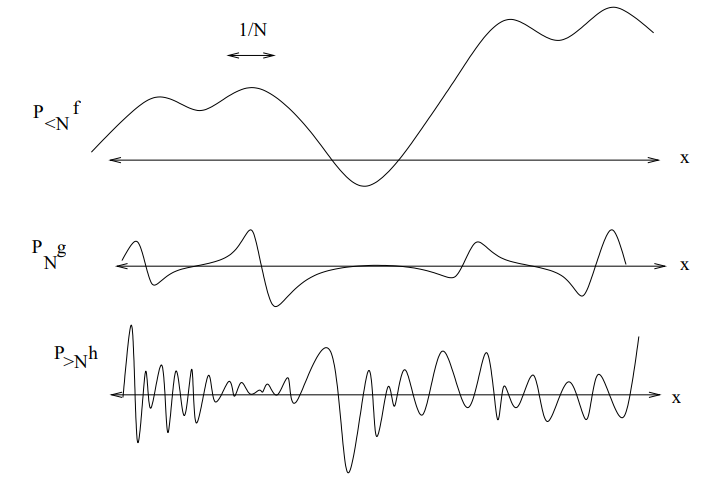
\includegraphics[scale =0.5]{uncertainty}
		\caption{Amplitudes of the projections to low, medium and high frequencies and their behavior at spatial scale $1/N$. This graphic is taken from \cite[Appendix A]{Tao2006}.}
	\end{center}
\end{figure}




\begin{proposition}[Local constancy for low frequencies]
	Let $k \in \N_0$, then 	
		\[ |\nabla^k f_{\leq N} (y)| \lesssim_{k, d} N^k \langle N(y - x) \rangle^d \cM f (x) \]
	uniformly for $f \in L^1_{\loc} (\R^d)$ and $N \in 2^\Z$. The analogous inequality holds replacing $f_N$ with $f_{\leq N}$. 
\end{proposition}

\begin{proof}
	By translation and scaling, we can assume without loss of generality that $x = 0$ and $N = 1$. The Littlewood-Paley projection can be written as a convolution with the kernel $\widecheck \phi \in \cS (\R^d)$. As the kernel and its derivatives are Schwartz, they can be bounded pointwise by $|\nabla^k \widecheck \phi (x)| \lesssim \langle x \rangle^{-100d}$. Thus
		\begin{align*}
			 |\nabla^k P_{\leq 1} f (y)|
			 	&\lesssim \int_{\R^d} \frac{|f(z)|}{\langle  y - z \rangle^{100d}} \, dz.
		\end{align*}	
	We divide the integral up into two regions. In the region $|z| \lesssim \langle y\rangle$, we crudely estimate
		\begin{align*}
			\int_{|z| \lesssim |y|}  \frac{|f(z)|}{\langle  y - z \rangle^{100d}} \lesssim \int_{|z| \lesssim |y|} |f(z)| \, dz \lesssim \langle y \rangle^d \cM f(0).
		\end{align*}
	In the region $|z| \gg \langle y\rangle$, the denominator can be estimated as $\langle y - z \rangle^{-100d} \sim \langle z \rangle^{-100d}$, then we decompose the region into dyadic annuli of radii $R \in 2^\N$ to write	
		\begin{align*}
			\int_{|z| \gg |y|} \frac{|f(z)|}{\langle  y - z \rangle^{100d}} \, dz
						&\lesssim \sum_{\substack{R \in 2^\N}} \int_{R \leq |z| \leq 2R} \frac{|f(z)|}{\langle z \rangle^{100d}} \, dz \\
						&\sim \sum_{\substack{R \in 2^\N}} R^{-100d}\int_{|z| \leq 2R} |f(z)| \, dz\lesssim \sum_{\substack{R \in 2^\N}} \langle R \rangle^{-99d} \cM f(0) \lesssim \cM f(0).
				\end{align*}
	This proves the pointwise inequality. 
\end{proof}

The fact that high frequencies have approximate mean zero on large balls is less useful, so we only sketch how to formalise the principle. Choose $\phi_{\lesssim N} \in \cS (\R^d)$ with disjoint Fourier support from $P_{\geq N} f$, then 
	\[ \int_{\R^d} \widecheck{\phi_{\lesssim N}} f_{\geq N} \, dx = 0 \]
by Plancharel. The inverse Fourier transform $\widecheck{\phi_{\lesssim N}} \in \cS (\R^d)$ is a Schwartz function adapted to the ball $B_{1/N} (0)$; modulating in frequency space allows us to adapt it to any ball $B_{1/N} (x_0)$. The mass outside of this ball, modulo scaling the radius by a constant, is negligible, hence
	\[ \int_{B_{C/N} (x_0)} f_{\geq N} \, dx \approx 0. \]

\subsection{Bernstein's inequalities}

There are two obstructions to moving between $L^p$-spaces: growth of singularities and decay at infinity. At one end, $L^\infty$-functions have no singularities and no decay at infinity, and at the other end, $L^1$-functions can have large singularities and a lot of decay at infinity. Projecting to low frequencies ``smooths'' the singularities, so we can ``pay'' some of this smoothing to control a higher $L^q$-space by a lower $L^p$-space. 

\begin{proposition}[Bernstein's inequalities]\label{prop:bernstein}
	For $1 \leq p \leq q \leq \infty$ and $f \in L^p (\R^d)$, then 
	\begin{align*}
					||f_N||_{L^q} 
						&\lesssim_{p, q} N^{\frac{d}{p} - \frac{d}{q}} ||f_N||_{L^p}, \\
					||f_{\leq N}||_{L^q} 
						&\lesssim_{p, q} N^{\frac{d}{p} - \frac{d}{q}} ||f_{\leq N}||_{L^p}. 
				\end{align*}
\end{proposition}

\begin{proof}
	Let $1 \leq r \leq \infty$ satisfy $\tfrac1p + \tfrac1r = \tfrac1q + 1$, then by Young's convolution inequality and a change of variables $Nx = y$, we have the inequality
	\begin{align*}
		|| P_N f ||_{L^q} = || f * \widecheck{\psi_N} ||_{L^p} \leq ||f||_{L^p} ||N^d \widecheck \psi(Nx)||_{L^r_x} = N^{d - \frac{d}{r}} ||f||_{L^p} ||\widecheck \psi ||_{L^r_y} \sim N^{\frac{d}{p} - \frac{d}{q}} ||f||_{L^p}.
	\end{align*}
	To obtain $f_N$ instead of $f$ on the right, observe that the same proof holds replacing $P_N$ with the fattened projection $\widetilde{P_N}$. Since $\widetilde{P_N} P_N = P_N$, replacing $f$ with $P_N f$ completes the proof. Arguing similarly furnishes the inequality replacing $f_N$ with $f_{\leq N}$. 
\end{proof}

\begin{remark}
	Compare with the dual phenomenon of localising in physical space, where if $1 \leq p \leq q \leq \infty$, applying Holder's inequality gives
		\[ ||\phi_{\leq N} f||_{L^p} \lesssim N^{\frac{d}{p} - \frac{d}{q}} ||\phi_{\leq N} f||_{L^q}. \]
	Applying a cut-off gives decay at infinity, which allows us to ``pay'' this decay to control a lower $L^p$-space by a higher $L^q$-space. 	
\end{remark}

\begin{remark}
	It is instructive to use the uncertainty principle to justify Bernstein's inequality. Suppose most of the $L^p$ and $L^q$-mass is located in a ball of radius $O(1)$, and recall low frequencies are locally constant at scales $\ll 1/N$. Hence we can approximate $f_{\leq N}$ by a function on the discrete space $N^d$, where we have the following discrete analogue of Bernstein's inequality,
		\[ ||f||_{\ell^q (N^d)} \lesssim N^{\frac{d}{p} - \frac{d}{q}} ||f||_{\ell^p (N^d)}. \]
\end{remark}


\subsection{Sobolev-Bernstein inequalities}

When applying for example the solid gradient $|\nabla|^s$ to a Littlewood-Paley projection and examining the symbol in frequency space, we can formally justify the following heuristics:
\begin{itemize}
	\item \textit{Low frequencies} are diminished by positive order differential operators and accentuated by negative orders, 
		\[ |\nabla|^s P_{\leq N} f \lesssim N^s P_{\leq N } f \qquad \text{for $s \geq 0$}.\] 
	
	\item \textit{High frequencies} are accentuated by positive order differential operators and diminished by negative orders,
		\[ |\nabla|^{s} P_{\geq N} f \lesssim N^{s}P_{\geq N} f \qquad \text{for $s \leq 0$}.\] 
	
	\item \textit{Medium frequencies} share the properties of both high and low frequencies,  	
		\[ |\nabla|^s P_{\leq N} f \sim N^s P_N f \qquad \text{for $s \in \R$}.\] 
\end{itemize}
These heuristics can be made rigorous to prove the \textit{Sobolev embedding inequalities}. Morally, if one can prove Sobolev embedding for a Littlewood-Paley piece, one can prove it for a generic function via summing. As such, we introduce


\begin{lemma}[Sobolev-Bernstein inequalities] For $f \in L^p (\R^d)$, 
				\begin{alignat*}{2}
					|| |\nabla|^s f_{\leq N}||_{L^p} 
						&\lesssim N^s ||f_{\leq N}||_{L^p}, &&\qquad\text{if }s > 0 \text{ and } 1 \leq p < \infty, \\
					|| |\nabla|^s f_{\geq N}||_{L^p} 
						&\lesssim N^s ||f_{\geq N}||_{L^p}, &&\qquad\text{if }s < 0 \text{ and } 1 \leq p < \infty \\
					|| |\nabla|^s f_N||_{L^p} 
						&\sim N^s ||f_N||_{L^p}, &&\qquad \text{if }s \in \R \text{ and } 1 \leq p \leq \infty
				\end{alignat*}			
		The endpoint cases $p = \infty$ for the first two inequalities hold for $f \in C_0 (\R^d)$. 
\end{lemma}

\begin{proof}
	Let 
		\[ \chi (\xi) := |\xi|^s \psi (\xi), \qquad \chi_N (\xi) := \chi (\xi/N). \]
	Observe that $\chi \in \cS (\R^n)$ since $\psi$ vanishes in a neighborhood of the origin. Then by Young's convolution inequality and the change of variables $Nx = y$, we have
		\[ || |\nabla|^s f_N||_{L^p} = || ({|\xi|^s \psi (\xi/N)})^{\vee} * f ||_{L^p} = N^s ||\widecheck{\chi_N} * f||_{L^p} \leq N^s ||f||_{L^p} ||N^d \widecheck{\chi} (N x)||_{L^1_x} = N^s ||f||_{L^p} ||\widecheck \chi(y)||_{L^1_y}. \]	
	The inequality continues to hold using instead the fattened Littlewood-Paley projections, so arguing as we did in Bernstein's inequality, we can replace $f$ with $f_N$ on the right-hand side. To obtain the reverse inequality, note the previous argument holds for the fattened projections. Hence, since Fourier multipliers commute and $\widetilde{P_N} P_N = P_N$,
		\[ ||f_N||_{L^p} = || |\nabla|^{-s} \widetilde{P_N} |\nabla|^s f_N||_{L^p} \lesssim N^{-s} || |\nabla|^s f_N||_{L^p}.  \]
	Rearranging furnishes the result. 	

	To prove the inequalities, we remark that the representation formulas $\sum_{K \leq N} f_K = f_{\leq N}$ and $\sum_{K \geq N} f_K = f_{\geq N}$ hold in $L^p (\R^d)$ for $1 < p < \infty$ and in the case $p = 1$ when $f$ has zero mean, see the following section for proofs. It follows from the triangle inequality that
		\[	|| |\nabla|^s f_{\leq N} ||_{L^p} \leq \sum_{K \leq N} || | \nabla|^s f_K||_{L^p} \sim \sum_{K \leq N} K^s ||f_K||_{L^p} \lesssim N^s ||f_{\leq N} ||_{L^p}\]
	for $s > 0$ and $1 \leq p < \infty$ and
		\[	|| |\nabla|^s f_{\geq N} ||_{L^p} \leq \sum_{K \geq N} || | \nabla|^s f_K||_{L^p} \sim \sum_{K \geq N} K^s ||f_K||_{L^p} \lesssim N^s ||f_{\geq N} ||_{L^p}\]
	for $s < 0$ and $1 \leq p < \infty$. 
\end{proof}


\subsection{Localised estimates}

When studying partial differential equations, we often times only want to look at a solution locally.  The standard way of doing this is to multiply by a cut-off function $\chi \in C^\infty_c (\R^d)$ adapted to a spatial ball of radius $R$. By the uncertainty principle, its Fourier transform should be adapted to a frequency ball of radius $R^{-1}$, thus multiplication by $\chi$ ``almost'' commutes with $P_N$ for $RN \gg 1$. Formally, 
	\[ [P_N, \chi] \approx O (N^{-1} \nabla \chi \widetilde{P_{\leq N}}).  \]

\begin{proposition}[Commutator estimate]
	Let $1 \leq p \leq \infty$ and $\chi \in C^\infty_c (\R^d)$ is a smooth cut-off. For $R > 0$, set $\chi_R (x) := \chi (x/R)$, then for any $k \geq 1$ we have 
		\[ || [P_N, \chi_R] f||_{L^p} \lesssim (RN)^{-1} ||\nabla \chi||_{L^\infty} || {P_{\leq 2N}} f||_{L^p} +  (RN)^{-k} || |\nabla|^k \chi||_{L^\infty}||f||_{L^p} .\]
\end{proposition}

\begin{proof}
	By scaling, assume without loss of generality $R  = 1$. We perform a paraproduct decomposition, inserting the expansions $\chi = \sum_A \chi_A$ and $f = \sum_B f_B$ and separating between high-low, high-high, and low-high interactions,
		\begin{align*}
			[P_N, \chi] f 
				&= P_N (\chi f) - \chi P_N f\\
				&= \left(\sum_{\substack{B \geq 4N \\ A \leq B/4}} + \sum_{\substack{B \geq 4N \\ A \geq B/2}} + \sum_{\substack{B \leq 2N \\ A \in 2^\Z}} \right) P_N (P_A \chi P_B f) - P_A \chi P_N P_B f.
		\end{align*}	
	Notice that the high-low summands vanish, since in this frequency regime $P_A \chi P_B f$ and $P_B f$ have Fourier supports at high frequencies $|\xi| \geq 2N$ and thus vanish when applying the projection $P_N$. For the high-high summand, again $P_N P_B f = 0$, while the term $P_A \chi P_B f$ can be dealt with by using smoothness of the cut-off to gain decay via Sobolev-Bernstein, 
		\begin{align*}
			 \sum_{\substack{B \geq 4N \\ A \geq B/2}} || P_N  (P_A \chi P_B f) ||_{L^p}
			 	&\lesssim \sum_{\substack{B \geq 4N \\ A \geq B/2}}  || | P_A \chi||_{L^\infty} || P_B f ||_{L^p} \\
			 	&\lesssim \sum_{\substack{B \geq 4N }} \sum_{A \geq B/2} A^{-k} || |\nabla|^k \chi||_{L^\infty} ||f||_{L^p}  \lesssim N^{-k} || |\nabla|^k \chi||_{L^\infty} ||f||_{L^p} . 
		\end{align*}	 
	It remains to estimate the low-high sum. Changing variables, we can write pointwise	
		\begin{align*}
			P_N (\chi P_{\leq 2N} f) (x) 
				&= \int_{\R^d} \widecheck \phi (y) \chi (x - y/N) P_{\leq 2N} f(x - y/N) \, dy,\\
			\chi P_N P_{\leq 2N} f (x)
				&= \int_{\R^d} \widecheck \phi (y) \chi (x) P_{\leq 2N} f (x - y/N) \, dy.
		\end{align*}
	By the fundamental theorem of calculus, we can estimate the difference $|\chi(x) - \chi(x - y/N)| \lesssim |y| N^{-1} ||\nabla \chi||_{L^\infty}$. It follows then from Minkowski's integral inequality and integrability of $y \widecheck \phi \in \cS (\R^d)$ that 
		\begin{align*}
			||P_N (\chi P_{\leq 2N} f) - \chi P_N P_{\leq 2N} f||_{L^p}
				&\leq N^{-1} ||\nabla \chi||_{L^\infty} ||P_{\leq 2N} f||_{L^p}.
		\end{align*}	
	This completes the proof. 
\end{proof}	

\begin{remark}
	The estimate can be further refined so that the $L^p$-norms on the right are localised by writing $\chi = \widetilde \chi \chi$, where $\widetilde \chi \equiv 1$ on the support of $\chi$. 
\end{remark}

In a similar spirit, we have a spatially localised version of Bernstein's inequality, see for example \cite{Tao2020} and \cite{Palasek2022} for applications to the Navier-Stokes equations: 

\begin{proposition}[Localised Bernstein's inequality]
	Let $\Omega \subseteq \R^d$ be a domain and $N \in 2^\Z$. For any $R \geq 1$ and $k \gg 1$, 
		\[ || P_N f ||_{L^{q_1} (\Omega)} \lesssim_{p_1, p_2, q_1, q_2, k} N^{\frac{d}{p_1} - \frac{d}{q_1}} ||f||_{L^{p_1} (B_R (\Omega))} + (RN)^{-k} |\Omega|^{\frac{1}{q_1} - \frac{1}{q_2}} N^{\frac{d}{p_2} - \frac{d}{q_2}} ||f||_{L^{p_2} (\R^d)}  \]
	whenever $1 \leq p_1 \leq q_1 \leq \infty$ and $1 \leq p_2 \leq q_2 \leq \infty$ such that $q_1 \leq q_2$. 
\end{proposition}

\begin{proof}
	We decompose $f = f \mathbb 1_{B_R (\Omega)} + f \mathbb 1_{\R^d \setminus B_R (\Omega)}$. The component supported on $B_R (\Omega)$ can be estimated by the first term on the right via Bernstein's inequality, it remains to show that $f =  f \mathbb 1_{\R^d \setminus B_R (\Omega)}$ supported on the complement $\R^d \setminus B_R (\Omega)$ is controlled by the second term on the right. By Holder's inequality, 
		\begin{align*}
			|| P_N f ||_{L^{q_1} (\Omega)} \leq |\Omega|^{\frac{1}{q_1} - \frac{1}{q_2}} || P_N f||_{L^{q_2} (\Omega)}. 
		\end{align*}
	For $x \in \Omega$, we can replace the kernel to its restriction to $|y| \geq R$, writing $P_N f(x) = (f * \mathbb 1_{|y| \geq R}\widecheck \psi_N) (x)$. Following the proof of Bernstein's inequality, we apply Young's convolution inequality and estimate $\widecheck \psi \in \cS (\R^d)$ by $|\widecheck \psi (y)| \lesssim_k \langle y \rangle^{-k}$, furnishing
		\[ ||P_N f||_{L^{q_2} (\Omega)} \leq  ||\widecheck \psi_N||_{L^r (|y| \geq R)} ||f||_{L^{p_2} (\R^d)} \lesssim_k (RN)^{-k} N^{\frac{d}{p_2} - \frac{d}{q_2}} ||f||_{L^{p_2} (\R^d)}.  \]
	This completes the proof. 
\end{proof}



\section{Littlewood-Paley square function}
Although the frequency supports of the Littlewood-Paley projections overlap, they nonetheless retain a degree of independence of one another in that one can multiply each projection of $f \in L^p (\R^d)$ by $\pm 1$ and the resulting function will still remain in $L^p (\R^d)$. This is encapsulated by the square function estimate; define the \emph{Littlewood-Paley square function} by
	\[ S(f) := ||f_N||_{\ell^2_N} = \Big( \sum_{N \in 2^\Z} |f_N|^2 \Big)^\frac12. \]	 
We claim that the $||f||_{L^p} \sim ||S(f)||_{L^p}$. The aforementioned independence suggests the following probabilistic approach:	

\begin{lemma}[Khinchine's inequality]
	Let $\{ X_n \}_n$ be i.i.d. random variables with $X_n = \pm 1$ with equal probability, then 
		\[ \Big( \EE \Big\{ \Big| \sum_n c_n X_n \Big|^p \Big\}  \Big)^\frac1p \sim_p \Big( \sum_n |c_n|^2\Big)^\frac12 \]
	for all $1 < p < \infty$ and $\{c_n\}_n \subseteq \C$. 	
\end{lemma}

\begin{proof}
	When $p = 2$, we have
		\begin{align*}
			 \EE \Big\{ \Big| \sum_n c_n X_n \Big|^2\Big\}
			 	&= \EE \Big\{ \Big( \sum_n c_n X_n \Big)\Big( \sum_m \overline{c_n} X_n \Big)\Big\} \\
			 	&= \sum_n |c_n|^2 \, \EE \{ X_n^2 \} + \sum_{m \neq n} c_n \overline{c_m} \, \EE\{X_n X_m\} = \sum_n |c_n|^2
		\end{align*}
	since $\EE\{X_n^2\} = 1$ and, by independence, $\EE \{X_n X_m\} = \EE \{X_n\} \EE \{X_m\} = 0$ whenever $m \neq n$. 	
	
	For the remaining $1 < p < \infty$, we assume without loss of generality $c_n \in \R$. By the layered cake decomposition, we can write
		\[ \EE \Big\{ \Big| \sum_n c_n X_n \Big|^p \Big\} = p \int_0^\infty \lambda^p \PP \Big\{ \Big| \sum_n c_n X_n \Big| > \lambda \Big\} \frac{d\lambda}{\lambda}. \]
	Moreover, 
		\[  \PP \Big\{ \Big| \sum_n c_n X_n \Big| > \lambda \Big\} = \PP \Big\{ \sum_n c_n X_n  > \lambda \Big\} + \PP \Big\{  \sum_n c_n X_n < - \lambda \Big\}. \]	
	We bound the first term on the right; arguing similarly will give the same bound on the second term on the right. It follows from the exponential Chebyshev inequality and independence that
		\begin{align*}
			\PP \Big\{ \sum_n c_n X_n  > \lambda \Big\}
				&\leq e^{-\lambda t} \EE \Big\{ e^{t \sum_n c_n X_n} \Big\} = e^{-\lambda t} \prod_n \EE \Big\{ e^{t c_n X_n} \Big\} =e^{-\lambda t} \prod_n \frac{e^{t c_n} + e^{- t c_n}}{2} = e^{-\lambda t} \prod_n \cosh (tc_n)
		\end{align*}	
	for any $t > 0$. Recalling that $\cosh x \leq e^{x^2/2}$	and choosing $t = \lambda /\sum_n |c_n|^2$ gives
		\[ \PP \Big\{ \sum_n c_n X_n  > \lambda \Big\} \leq  e^{-\lambda^2/2\sum_n |c_n|^2} .\]
	Returning to the layered cake decomposition, making a change of variables $\alpha = \lambda /(\sum_n |c_n|^2)^{1/2}$, we obtain
		\[  \EE \Big\{ \Big| \sum_n c_n X_n \Big|^p \Big\} \leq 2p \int_0^\infty \lambda^p e^{-\lambda^2/2 \sum_n |c_n|^2} \frac{d\lambda}{\lambda} = 2p \Big(\sum_n |c_n|^2 \Big)^{\frac{p}{2}} \int_0^\infty \alpha^p e^{-\alpha^2/2} \frac{d\alpha}{\alpha} \lesssim_p \Big(\sum_n |c_n|^2 \Big)^{\frac{p}{2}}. \]	
	For the reverse inequality, it follows from Holder's inequality and the inequality above that
		\begin{align*}
			 \sum_n |c_n|^2 = \EE \Big\{ \Big| \sum_n c_n X_n \Big|^2 \Big\} &\leq \Big( \EE \Big\{ \Big|\sum_n c_n X_n \Big|^p \Big\} \Big)^\frac1p \Big( \EE \Big\{ \Big|\sum_n c_n X_n \Big|^{p'} \Big\} \Big)^\frac{1}{p'} \\
			 & \lesssim \Big(\sum_n |c_n|^2 \Big)^\frac12 \Big( \EE \Big\{ \Big|\sum_n c_n X_n \Big|^p \Big\} \Big)^\frac1p.  
		\end{align*}	 
	Rearranging furnishes the result. 	 
\end{proof}

\begin{theorem}[Littlewood-Paley square function estimate]\label{thm:square}
	For $1 < p < \infty$ and $f \in L^p (\R^d)$, we have
		\[ || S(f)||_{L^p} \sim ||f||_{L^p}. \]
\end{theorem}

\begin{proof}
	Let $\{X_N\}_{N \in 2^\Z}$ be i.i.d with $X_N = \pm 1$ with equal probability. By Khinchine's inequality, 
		\[ \EE \Big\{ \Big|\sum_{N \in 2^\Z} f_N X_N \Big\}\Big|^p  \sim |S(f)|^p. \]
	Then 
		\[ ||S(f)||_{L^p}^p \sim \int_{\R^d} \EE \Big\{ \Big|\sum_{N \in 2^\Z} f_N X_N \Big|^p \Big\} dx. \]	
	We claim that $m (\xi) := \sum_N X_N \psi_N (\xi)$ is a Mikhlin multiplier uniformly with respect to choice of $X_N$. Indeed, since $\psi (\xi)$ is localised about $|\xi| \sim 1$, we obtain
		\[ |\partial^\alpha_\xi m (\xi)| \leq \sum_{N \in 2^\Z} |\partial^\alpha_\xi \psi_N (\xi)| \lesssim \sum_{N \in 2^\Z} N^{-|\alpha|} |\partial^\alpha_\xi \psi(\xi/N)| \sim \sum_{|\xi| \sim N} N^{-|\alpha|} \lesssim |\xi|^{-|\alpha|}.  \]
	Thus
		\[ ||S(f)||_{L^p}^p \sim \EE \{ || m(\nabla) f ||_{L^p}^p \}\lesssim \EE \{ ||f||_{L^p}^p \} = ||f||_{L^p}^p. \]	
	For the reverse inequality, we argue by duality and the fattened projections. Denote $\widetilde S(f)$ the fattened square function, i.e. replacing the projections $P_N f$ with the fattened projections $\widetilde{P_N} f$. The inequality above continues to hold replacing $S$ with $\widetilde S$. We write
	\begin{align*}
		||f||_{L^p}
			&= \sup_{||g||_{L^{p'}} = 1} \langle f, g \rangle = \sup_{||g||_{L^{p'}} = 1} \sum_{N \in 2^\Z} \langle \widetilde{P_N} P_N f, g \rangle = \sup_{||g||_{L^{p'}} = 1} \sum_{N \in 2^\Z} \langle  P_N f, \widetilde{P_N} g \rangle \\
			&\leq  \sup_{||g||_{L^{p'}} = 1} \langle S(f), \widetilde{S} (g) \rangle \leq  \sup_{||g||_{L^{p'}} = 1} || S(f) ||_{L^p} ||\widetilde{S}(g)||_{L^{p'}} \lesssim ||S(f)||_{L^p},
	\end{align*}
	where the second equality holds since $f =\sum_N \widetilde{P_N} P_N = \sum_N P_N f$ in $L^p (\R^d)$, the third equality holds by self-adjointness of Fourier multipliers, the first inequality holds by Cauchy-Schwartz in $N$, the second by Holder in $x$, and the third by the square function inequality for the fattened projections. 
\end{proof}	

\begin{remark}
	The estimate fails at the endpoints. For $p = \infty$, taking $f = 1$, we have $f_N = 0$ and therefore $S(f) = 0$. For $p = 1$, take $f = \phi_\epsilon$ where $\{\phi_\epsilon\}_\epsilon \subseteq C^\infty_c (\R^d)$ is an approximation to the identity. 
\end{remark}


\bibliographystyle{alpha}
\bibliography{external/biblio}

\end{document}